\section{New Graph--based Syntax}
The ultimate goal of the new graph--based syntax presented here is to be able to 
fully describe the fundamental problem formulation for a complex design task, 
while still being able to accomodate the more specific case when a solution 
strategy is applied to the problem formulation. In order to achieve that goal 
the graph needs to accomodate a number of constructs from MDAO problem: 

\begin{itemize}
    \item Analysis tools 
    \item Local and global variables 
    \item Coupling between analyses
    \item Design variables
    \item Objective or objectives 
    \item Local and global Constraints
    \item Iterative loops from solvers and optimizers
\end{itemize}

The following section provides an overview of graph theory basics, then describes 
in detail the different node and edge types, as well as rules governing allowable 
egdegs between nodes, used as the foundation of the new graph syntax. These basic graph 
primatives are them mapped to the MDAO constructs stated above, and used to 
build three distinct graph forms: 

\begin{itemize}
    \item Maximal Connectivity
    \item Fundamental Problem Formulation 
    \item Specific Solution
\end{itemize}

Each of these forms serves a different purpose in the design process, and we 
present some transformations that can be applied to transition 
between any two of the three graph forms. 

\subsection{Graph Theory Basics}
The notation used in this work is adapted from Diestel \cite{Diestel2010}. 
A \emph{graph} is a pair $G = (V,E)$ of sets such that $E \subseteq V \times V$, 
which means that the elements of $E$ are 2--element subsets of $V$. The set $V$ 
contains the \emph{vertices} or \emph{nodes} and the set $E$ contains the \emph{edges}.
For a \emph{directed graph*} we construct $E$ as a set of ordered pairs instead 
of a set of sets. Each ordered pair represents an edge starting at the node 
indicated by the first entry and directed to the node indicated by the second 
entry. Edge $e$ = $(x,y)$ may be referred to simply as $xy$ and we say $y = E(x)$. 

\begin{figure}[htb!]
	\begin{center}
	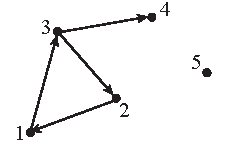
\includegraphics[width=1.5in]{images/example_directed_graph}
	\end{center}
	\vspace{-20pt}
\caption{Example directed graph.}
\label{f:example directed graph}
\end{figure}
As an example, for the directed graph shown in Fig.~\ref{f:example directed graph} we have
\begin{IEEEeqnarray*}{rCl}
V & = & \{1,2,3,4,5\}, \\
E & = & \big\{(1,2),(3,2),(1,3),(3,4)\big\}.
\end{IEEEeqnarray*}

% \subsection{Problem Formulation Concepts to Represent}
% The MDAO problem formulation concepts we wish to represent are:
% \begin{description}
% \item[global input] A global input is a variable that is taken as given and is used by multiple analyses.
% \item[design variable]
% \item[function call] A function call requires a set of inputs to be fulfilled and has certain properties, such as run time, which are independent of the number of outputs actually being used.
% \item[passing of distinct variables] Instead of connecting analyses, the individual variables as are connected
% \item[objective \& constraint] These are variables that must be produced by the problem formulation for it to be valid
% \item[collision] A collision occurs when an input has multiple sources
% \item[hole] A hole occurs when an input has no sources
% \item[coupling] Couple is the mutual dependence between a set of analysis
% \item[multi--fidelity] It may be desirable for the same variable to be calculated by separate analyses and to use both results.
% \end{description}

\subsection{MDAO Graph Primatives}
There are three node types:  
\begin{description}
\item[variable node] represents passing of data.
\item[model node] represents the handling of data.
\item[driver node] represents constrol structures capable of managing iteration
\end{description}
There are two edge types: 
\begin{description}
\item[fixed edge] A fixed edge may never be removed from the graph.
\item[free edge] A free edge may be removed removed from the graph.
\end{description}

A number of restrictions are places on the model node with respect to the number and 
type of edges that can be connected to it: 
\begin{enumerate}
\item A model node can only have one edge directed to or from another model node.
\item A model node can only have fixed edges directed in or out.
\item A model node must have at least one edge directed in and at least one edge directed out.
\end{enumerate}

Analysis tools take in a number input variables, then perform some work calculate 
the values for their respective outputs. In an MDAO graph, this process is 
represented by an group of nodes and edges called an \emph{analysis block}, 
shown in Fig. \ref{f:analysis block}. Within an analysis block each variable 
node represents a single input or output and is connected 
to a single model node via a fixed edge. Note that in Fig. \ref{f:analysis block}, 
the analysis block contains two model nodes, with a single edge connecting them. 
This part of the graph represents the necessary calculations to map given inputs 
to proper output values. 

\begin{figure}[htb!]
    \begin{center}
    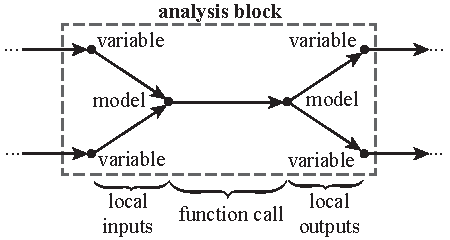
\includegraphics[width=4in]{images/analysis_block}
    \end{center}
    \vspace{-10pt}
\caption{Example analysis block. The each node type and edge type is labeled in italics and annotated parenthetically.}
\label{f:analysis block}
\end{figure}

Finally, free edges are used to connect the variable nodes of the analysis block 
to other variables nodes outside of the analysis block. In this way, the 
analysis block graph is a fundamental building block of the MDAO problem data flow.


The MDO problem formulation concepts represented by nodes are given in 
Table \ref{t:node representation}, and the concepts represented by edges are 
given in Table \ref{t:edge representation}.
% \begin{itemize}
% \item An objective or constraint is indicated by a variable node with no outgoing edges and with the incoming edges being directed from only other variable nodes.
% \item A global input is a variable node with no edges directed in and with at least two edges directed out to different variable nodes.
% \item A design variable is represented by a variable node with no edges directed in and on fixed edge directed out.
% \end{itemize}
\begin{table}[h!]
 \begin{center}
  \caption{Problem formulation concept represented by a node}
  \label{t:node representation}
  \begin{tabular}{ccc} \hline 
edges directed in & edges directed out & node representation \\ \hline
only free edges & none & objective or constraint\\
none & at least two free edges & global input \\
none & one fixed edge & design variable \\ \hline
  \end{tabular}
 \end{center}
 \vspace{-15pt}
\end{table}
\begin{table}[h!]
 \begin{center}
  \caption{Problem formulation concept represented by an edge}
  \label{t:edge representation}
  \begin{tabular}{ccc} \hline 
from node & to node & edge representation \\ \hline
variable & variable & connection/passing of a variable\\
variable & model & local input \\
model & variable & local output \\
model & model & function call \\ \hline
  \end{tabular}
 \end{center}
 \vspace{-15pt}
\end{table}
%`Connection' edges connect the local outputs from one analysis block to input nodes.

\section{Graph--based Representation of the Fundamental Problem Formulation}
Next we provide the meaningful graphs that can be created from the suggested syntax. The first graph is the \emph{maximal connectivity graph} which represents the full potential of all the analysis codes being considered, i.e. each analysis code is represented by an analysis block, and each potential connections between variables is represented by a free edge. The second graph that may be represented is \emph{fundamental problem formulation graph}, which is the graph with the fewest number of edges and nodes needed to provide a valid problem formulation, as disscussed subsequently. Finally, a \emph{solution problem formulation} may be represented by including additional edges and node times to represent the optimization architecture, though this is beyond the scope of this paper. 

The relationship between these three graphs is depicted in Figs.~\ref{f:tree} and \ref{f:hourglass}. The tree diagram demonstrates the fact that it is generally possible to obtain multiple FPFs from a single maximal connectivity graph. This  may correspond to different down--selections of analysis codes, different connections between them, or both. Then, for each FPF, different SPFs may be obtained by implementing different optimization architectures. The hourglass shape indicates that the FPF graph is the smallest graph that may represent a specific problem formulation. The FPF is obtained from the MCG by removing nodes and edges, and the SPF is obtained from the FPF by adding nodes and edges.
\begin{figure}[htb!]
	\centering
	\subfigure[number of possible graphs]{
	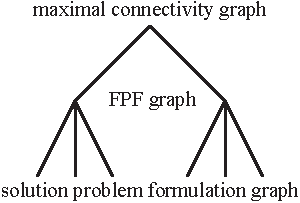
\includegraphics[width=2.0in]{images/tree}
	\label{f:tree}
	}
	\subfigure[graph size]{
	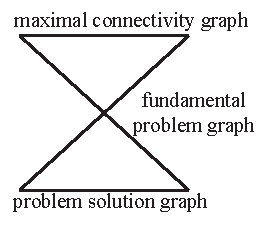
\includegraphics[width=2.0in]{images/hourglass}
	\label{f:hourglass}
	}
\caption{The relationship between the MCG, FPF, and SPF.}
\end{figure}

In this section we introduce the remaining necessary notion and give graph--theory based definitions of the MCG and FPF, and then process to demonstrate how the FPF is obtained from the MCG.

\subsection{Additional Notation}
For node $v \in V$ the edges directed out are given by $E(v)$ and the edges directed into $v$ are given by $E^{-1}(v)$; $E(E(v))$ is denoted as $E^2(v)$, and likewise for additional levels. 
The \emph{indegree} of a node is the number of edges directed in and is denoted as $\txt{deg}^-(v)$, and the \emph{outdegree} is the number of edges directed out and it is denoted as $\txt{deg}^+(v)$.
We also define the \emph{upper indegree limit} 
\begin{equation}
\txt{deg}_u^-(v):V \to \mathbb{N}
\end{equation} 
and the \emph{lower indegree limit}
\begin{equation}
\txt{deg}_l^-(v):V \to \mathbb{N}.
\end{equation}
These user-specified limits set the number of edges that may be directed into a node for a problem formulation to be valid. For example, a variable node $v$ will have $\txt{deg}_u^-(v) = \txt{deg}_l^-(v) = 1$, unless it is a multi--fidelity variable, in which case the user may specify some upper limit higher than one.

To keep track of which nodes and edges are which type, let $T_\txt{node}$ and $T_\txt{edge}$ be sets containing the possible node types and edge types, respectively, and then define mappings $t_\txt{node}:V \to T_\txt{node}$ and $t_\txt{edge}:E \to T_\txt{edge}$ to assign a type to each node and edge.
Then, for example, for a variable node $v$ we have $t_\txt{node}(v) = \txt{`variable'}$.


 % A \emph{path} is a nonempty graph $P = (V,E)$ with $V = \{x_0,x_1,\ldots,x_k\}$ and $E = \{x_0x_1,x_1x_2,\ldots,x_{k-1}x_k\}$, where $x_i$ are all distinct. A graph $G$ is \emph{connected} if any two of its vertices are linked by a path in $G$. A \emph{tree} is a connected and acyclic graph.
%%% this needs to be changed to fit the definition using a directed graph


\subsection{Maximal Connectivity Graph}
To construct the maximal connectivity graph, we assume that a set of codes, global inputs, and objectives and constraints (collectively called global outputs). The codes are represented by analysis blocks $A_i=(V_{A_i},E_{A_i}), \ i=1,\ldots,m$, the global inputs are represented a set of variable nodes $I$, and the global outputs are represented by a set of variable nodes $O$. We assume that $O$, $I$, and $A_i$ are given, and that any potential connection between variables is given in the form of the free edges in the set $C_M$. 
Then we may construct the maximal connectivity graph $M=(V_M,E_M)$ as
\begin{IEEEeqnarray*}{rCl}
V_M & = & I \cup O \cup \left( \bigcup_{i = 1}^m V_{A_i} \right), \\
E_M & = & C_M \cup \left( \bigcup_{i=1}^m E_{A_i} \right),
\end{IEEEeqnarray*}
The MCG $M$ is uniquely determined by the given set of analysis blocks, the required outputs, and the given global inputs. In the cases where the set of global inputs $I$ is not known a priori, the process of obtaining the FPF will reveal the required inputs, as discussed subsequently.

\subsection{Fundamental Problem Formulation Graph}
We now define the fundamental problem formulation graph, $F=(V_F,E_F)$, as a directed graph meeting the following conditions
\begin{enumerate}
\item[(1)] $\displaystyle{V_F = I_F \cup O \cup \left( \bigcup_{i \in \mathcal A} V_{A_i} \right),\ I_F \subset I}$
\item[(2)] $\displaystyle{E_F = C_F \cup \left( \bigcup_{i \in \mathcal A} E_{A_i} \right)}$
\item[(3)] $\displaystyle{\forall v \in V_F \txt{ with } t_\txt{node}(v) = \txt{`variable,'}\quad \txt{deg}_l^-(v) < \txt{deg}^-(v) \leq \txt{deg}_u^-(v)}$
\end{enumerate}
The set $\mathcal A$ is an index set containing the indices of the analysis blocks in $F$; for the case where all of the analysis blocks are used, we would have $\mathcal A = \{1,2,\ldots,m\}$. The first requirement for $F$ is that $V_F$ be composed of all of the global outputs (the required objectives and constraints), the nodes from each analysis block in $F$, and any global input nodes that are needed, $I_F$. The second requirement suggests that the edges in $F$ comprise the edges for each analysis block and the edges between them, the global inputs, and the global outputs. The final requirement is specific to the number of edges directed into a variable. If there are no edges directed inward, the node is called a \emph{hole}, and if more connections are directed in than are allowed, the node is called a \emph{collision}; a hole is allowed if $\txt{deg}_l^-(v)=0$. The final requirement is therefore a requirement on $C_F$.

\subsection{Obtaining the Fundamental Problem Formulation Graph}
In general, there may be multiple different graphs that satisfy the FPF conditions, though there may be none at all. Here, we describe a process for obtaining an FPF by starting with the MCG and disconnecting free edges until the FPF conditions are met. Then the problem is reduced to deciding which free edges to remove.

%Then, mathematically, the FPF starts with $\mathcal A_1 = \{1,\ldots,m\}$, $I_{F,1} = I$, and $C_{F,1} = C_M$.
Then, mathematically, the FPF starts with $C_{F,0} = C_M$.
First address the nodes where $\txt{deg}^-(v) < \txt{deg}_l^-(v)$ then the ones where $\txt{deg}^-(v) > \txt{deg}_u^-(v)$

\begin{enumerate}
\item The first step is to detect holes and disconnect the free edges following them. These free edges are removed because they represent variables which cannot be determined because the analysis function does not have adequate inputs. The set of variable nodes which are holes is created as
\begin{equation}
H = \{v \in V | \txt{deg}^-(v) < \txt{deg}_l^-(v) \}
\end{equation}
Then the updated set of edges is
\begin{equation}
C_{F,1} = C_{F,0} \setminus \{\ e \in E, \ e=xy | x=E^3(v) \txt{ for } v \in H\}
\end{equation}
%deg-v is now recaculated for the new C. 
This step is demonstrated by Fig.~\ref{f:holes}.
\item (())
\end{enumerate}
\begin{figure}[htb!]
	\begin{center}
	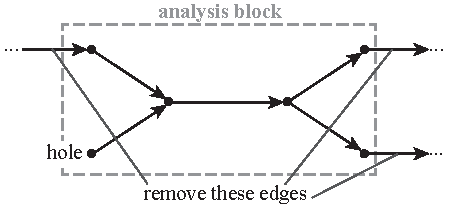
\includegraphics[width=3in]{images/analysis_block_hole}
	\end{center}
	\vspace{-20pt}
\caption{Example variable node indicating a hole.}
\label{f:holes}
\end{figure}


%\begin{enumerate}
%\item The first step is to detect holes and remove the corresponding analysis blocks, which could not be used because the required inputs are not supplied. Any analysis blocks with holes may be stored in an index set $\mathcal H$ as
%\begin{equation}
%\forall i \in \mathcal A_1,\txt{ and }\forall v \in V_{A_i},\txt{ if deg}^-(v)=0 \txt{ then } i \in \mathcal H.
%\end{equation}
%Then an updated index set $\mathcal A_2$ is created using set difference notation as
%\begin{equation}
%\mathcal A_2 = \mathcal A_1 \setminus \mathcal H
%\end{equation}The connection edges directed from the removed analysis blocks are removed as
%\begin{equation}
%H = \{c \in C_{F,1} |c = (e^{-1}(v),v), \txt{ where } v \in V_{A_i} \txt{ for some } i \in \mathcal H\},
%\end{equation}
%\begin{equation}
%C_{F,2} = C_{F,1} \setminus H
%\end{equation}
%Finally, the FPF is updated as
%\begin{equation}
%V_{F,2} = I_{F,2} \cup O \cup \left( \bigcup_{i \in \mathcal A_2} V_{A_i} \right),
%\end{equation}
%\begin{equation}
%E_{F,2} = C_{F,2} \cup \left( \bigcup_{i \in \mathcal A_2} E_{A_i} \right)
%\end{equation}
%This process may require multiple iterations because removing an analysis block may create holes upstream. It is assumed that the process as been repeated sufficiently such that $\mathcal A_2$ does not have any holes.
%
%\item The next step is to resolve conflicts. The set $C$ of input nodes containing conflicts is
%\begin{equation}
%C = \{v \in V_{F,2} | t_\txt{node}(v) = \txt{`input'} \txt{ and } \txt{deg}^-(v) > d(v)\}
%\end{equation}
%%\begin{equation}
%%for v \in c let 
%%\end{equation}
%\end{enumerate}

%\subsection{Classification of the FPF}

%A collision represents a choice.
%Delete edges and analysis blocks so that there are no nodes or collisions.





% \begin{figure}[htb!]
	% \begin{center}
	% 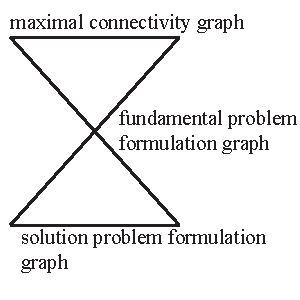
\includegraphics[width=2in]{images/hour_glass}
	% \end{center}
	% \vspace{-20pt}
% \caption{(()).}
% \label{f:our glass}
% \end{figure}
% \subsection{old}
	% For a large scale problem with many analyses, obtaining the FPF is likely to be a challenge. In general, a set of analysis codes will be given and the desired outputs will be specified as
	    % \begin{align}
            % given & \ \ A: \lbrace x_i \lvert i \in A_\textrm{input} \rbrace \rightarrow \lbrace x_i \lvert i \in A_\textrm{output} \rbrace \notag
            % \\    & \ \ B: \lbrace x_i \lvert i \in B_\textrm{input} \rbrace \rightarrow \lbrace x_i \lvert i \in B_\textrm{output} \rbrace \notag
			% \\    & \ \ \quad \quad \quad \quad \quad \quad  \quad \quad \vdots
            % \\min. &\ \ f(x_i), i \in \mathcal{O} \notag
            % \\w.r.t. & \ \ x_i, i \in \mathcal{I}, \notag
            % \label{eqn:preFPF}
        % \end{align}
	% where $\mathcal{O}$ is the index set of the global outputs and $\mathcal{I}$ is the index set of the global inputs. For this to be an FPF, there must be no \emph{conflicts} or \emph{holes}. A conflict arises when different analyses produce the same output; two analysis codes $A$ and $B$ are in conflict if
		% \begin{equation}
			% A_\textrm{output} \cap B_\textrm{output} \neq \emptyset.
		% \end{equation}
	% A hole arises when a local input to an analysis block is neither a global input nor a local output of any analysis block. If we let $\mathcal{H}$ denote the index set of local inputs which are holes
		% \begin{equation}
			% i \in \bigcup \{A_\textrm{input},B_\textrm{input},\ldots\} \textrm{ and } i \notin \bigcup \{\mathcal{I},A_\textrm{output},B_\textrm{output},\ldots\}  \implies  i \in \mathcal{H}.
		% \end{equation}
	% If the given set of analyses contains any holes, an FPF cannot be obtained. On the contrary, if there are conflicts multiple FPFs may be obtained. This is because every conflict represents a choice of which analysis to use and each choice could (potentially) yeild a different but valid FPF. The following section develops an application of graphy theory to obtain multiple FPFs from a set of analyses and desired outputs.
		
    % \subsection{Formulation Graph Syntax}
    % Rather than start with an adjacency, we chose to work directly with a directed cyclic graph to develop a syntax for the FPF. 
    % The following information must be provided to start:
    % \begin{itemize}
        % \item Analysis blocks: an analysis block represents any calculation, and each comes with
            % \begin{itemize}
                % \item local inputs
                % \item local outputs 
                % \item execution properties: these are the properties associated with running the code, such as run time
            % \end{itemize}
        % \item Global parameters: these may serve as fixed inputs to the local inputs of analysis blocks
        % \item Global outputs: these may represent
            % \begin{itemize}
                % \item objectives
                % \item constraints
                % \item residuals: (not sure)
            % \end{itemize}
    % \end{itemize}

    % The graph representation of a data flow is cast to utilize the extensive library of algorithms in graph theory to analyze a directed weighted graph. 
    % Edge weights are used to represent the metrics associated with a data flow:
    % \begin{itemize}
        % \item Run time: this metric is a property of an analysis block
        % \item Fidelity: this metric is a property of an individual local output
        % \item Expected Convergence
    % \end{itemize}

    % The key assumption is that identical variables are recognized as such. This serves as the basis for creating a data flow by connecting compatible input and output nodes with a directed edge. 
    % To represent the fact that execution of an analysis code does not depend on the number of outputs being used, we have created the following figure (not made yet).
    
    % This information immediately leads to the maximal connectivity graph, which is formed by placing a directed edge from each local output or global parameter to each matching local input or global output. 
    % Whenever multiple edges are connected to a single input, a conflict occurs because only one may be used. Resolving these conflicts is one key challenge in creating a data flow.
%    \begin{itemize}
%        \item Specify analyses
%        \item Connections between analyses 
%            \begin{itemize}
%                \item local variables
%                \item global variables? Use "fake" node that broadcasts out to the rest of the graph? 
%            \end{itemize}
%        \item Cycles indicate coupling
%        \item Cycles for design variables->objectives/constraints
%        \item Objectives/constraints are just outputs? Special nodes? 
%        \item Residuals are just outputs? Special nodes? 
%        \item Parameters are just input nodes that are not design variables (use identifies these)
%        \item FPF no solvers/optimizers anywhere in it
%    \end{itemize}

    \subsection{Solution Graph Syntax}
    What is the difference between a problem formulation and a problem solution method? Convert from a cyclic graph, to an acyclic graph
    \begin{itemize}
        \item Cycles indicate convergence loops or design variable loops
        \item Problem can't be solved until all loops are *removed* by adding solvers/optimizers
        \item *Special* nodes for solvers and optimizers that *break* loops (from an algorithmic point of view)
        \item FPF represents the minimal amount of information necessary to define a problem
        \item Any solution path grows the graph complexity by adding edges and nodes (or possibly have an empty solution graph, which you build up
        as you remove edges from problem formulation graph?)
    \end{itemize}
